\begin{marginfigure}[1cm]
\margingraphics{figures/1_6_PA1.eps}
\caption{The graph of $y = s(t)$, the position of the car (measured in thousands of feet from its starting location) at time $t$ in minutes.} \label{fig:2.3.PA1}
\end{marginfigure}

\begin{pa} \label{PA:2.3}
The position of a car driving along a straight road at time $t$ in minutes is given by the function $y = s(t)$ that is pictured in Figure~\ref{fig:2.3.PA1}.  The car's position function has units measured in thousands of feet.  For instance, the point $(2,4)$ on the graph indicates that after $2$ minutes, the car has traveled $4000$ feet.

\ba
	\item In everyday language, describe the behavior of the car over the provided time interval.  In particular, you should carefully discuss what is happening on each of the time intervals $[0,1]$, $[1,2]$, $[2,3]$, $[3,4]$, and $[4,5]$, plus provide commentary overall on what the car is doing on the interval $[0,12]$.
	\item On the lefthand axes provided in Figure~\ref{fig:2.3.PA1b}, sketch a careful, accurate graph of $y = s'(t)$.
	\item What is the meaning of the function $y = s'(t)$ in the context of the given problem?  What can we say about the car's behavior when $s'(t)$ is positive?  when $s'(t)$ is zero?  when $s'(t)$ is negative?
	\item Rename the function you graphed in (b) to be called $y = v(t)$.  Describe the behavior of $v$ in words, using phrases like ``$v$ is increasing on the interval $\ldots$'' and ``$v$ is constant on the interval $\ldots$.''
	\item Sketch a graph of the function $y = v'(t)$ on the righthand axes provide in Figure~\ref{fig:2.3.PA1b}.  Write at least one sentence to explain how the behavior of $v'(t)$ is connected to the graph of $y=v(t)$.
\ea

\end{pa} 

\begin{figure}
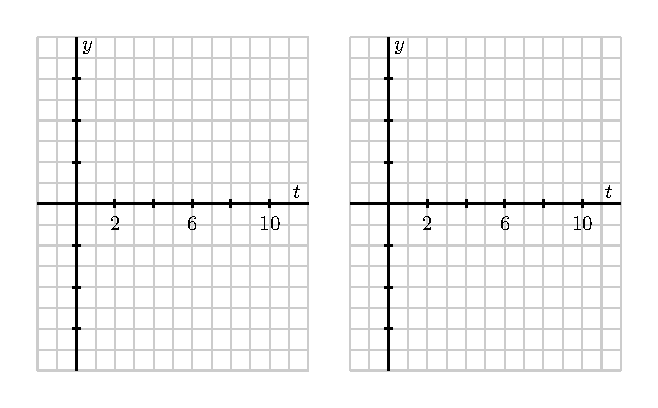
\includegraphics{figures/1_6_PA1b.eps}
\caption{Axes for plotting $y = v(t) = s'(t)$ and $y = v'(t)$.} \label{fig:2.3.PA1b}
\end{figure}

\afterpa

